\section{Wzory}

\subsection{Funkcje}

    \textbf{Liniowa:} $$f(x)=ax+b$$
    \textbf{Kwadratowa:} $$f(x)=ax^2+bx+c$$

\subsection{Ulamki}

    $$\frac{ \frac{15+x^{-3}}{x+1} }
    {\frac{\log(x^2)}{x+
    \frac{x^2}{15-x}}} =
    \frac{1}{x+ \frac{2}{1\frac{3}{x}}}$$

\subsection{Znak sumy}

    $$\sum_{i=1}^n{RX_i-Y_i}^2$$

\subsection{Granice}

    $$lim_{x\to 0}{\frac{e^x-1}{2x}}
    ={\left[\frac{0}{0}\right]}$$

\begin{figure}
    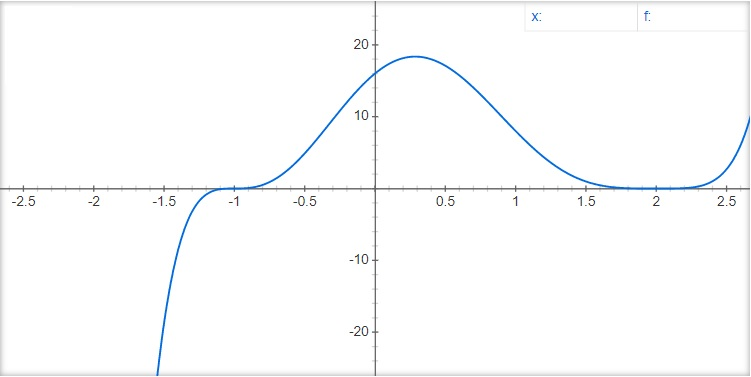
\includegraphics[angle=90,width=40mm]{wykres1}
    \caption{$f(x)=(x-2)^4(x+1)^3$}
\end{figure}

\begin{figure}
    \centering
    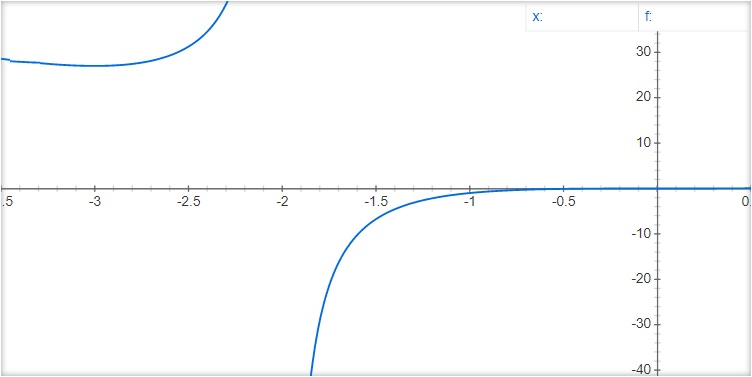
\includegraphics[width=50mm,height=!]{wykres2}
    \caption{$f(x)=\frac{x^3}{(x+2)}$}
\end{figure}
\begin{figure}
    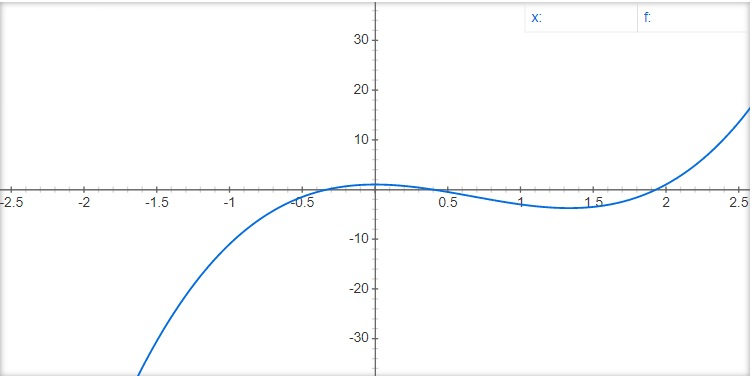
\includegraphics[angle=45,width=50mm]{wykres3}
    \caption{$f(x)=(x-2)^4(x+1)^3$}
\end{figure}